\documentclass[12pt,a4paper]{article}
\usepackage[polish]{babel}
\usepackage[T1]{fontenc}
\usepackage[utf8x]{inputenc}
\usepackage{hyperref}
\usepackage{url}
\usepackage{graphicx}
\usepackage{listings}
\usepackage{amsmath}
\usepackage{indentfirst}
\usepackage[]{algorithm2e}
\addtolength{\hoffset}{-1.5cm}
\addtolength{\marginparwidth}{-1.5cm}
\addtolength{\textwidth}{3cm}
\addtolength{\voffset}{-1cm}
\addtolength{\textheight}{2.5cm}
\setlength{\topmargin}{0cm}
\setlength{\headheight}{0cm}
\lstset{
  breaklines=true
}
\begin{document}
	
	\title{Dokumentacja projektu\\ Języki Skryptowe}
	\author{Arkadiusz Kałuża, gr. 2C}
	\date{\today}
	
	\maketitle
	\newpage
	\section*{Część I}
	\subsection*{Opis programu}
	Projekt spełnia warunki zadania Kłopot Rowerzysty z konkursu Algorytmion2014, dodatkowo obsługiwany jest z poziomu powłoki systemu Windows(skrypt napisany jest w języku Batch) oraz wyświetla wyniki wykonanych operacji na stronie internetowej. 
	\\
	\\ \indent Poniżej polecenie z konkursu Algorytmion:
	Na  samym  dole  koła  rowerowego  o  danym  promieniu Rsiedzi  mucha.  Rower przejechał n metrów. Napisz program obliczający (po zapytaniu o R i n) długość drogi, jaką  przebyła  w  tym  czasie  mucha  (zakładamy,  że  poruszała  się  ona    na  kole  nie zmieniając na nim swej pozycji). \\
\textbf{Uwaga 1.}
	 \\Można skorzystać z równania cykloidy.\\ 
\textbf{Uwaga 2.}
	 \\Długość  krzywej  można  przybliżać  długością  łamanej,  której  				wierzchołki znajdują się na tej krzywej (oczywiście im więcej 					wierzchołków, tym lepiej). Kierując się tą wskazówką, należy 					uwzględnić ilość wierzchołków jakoargument programu.\\
\textbf{Uwaga 3.}
	 \\Do rozwiązania (program) należy dołączyć opis rozwiązania problemu.\\
	 
Na poniższym rysunku znajduje się ilustracja zadania (szarym kołem zaznaczone są początkowa,  przejściowe i końcowa pozycja muchy, a pogrubiony niebieski łuk jest drogą przebyłą przez muchę.\\
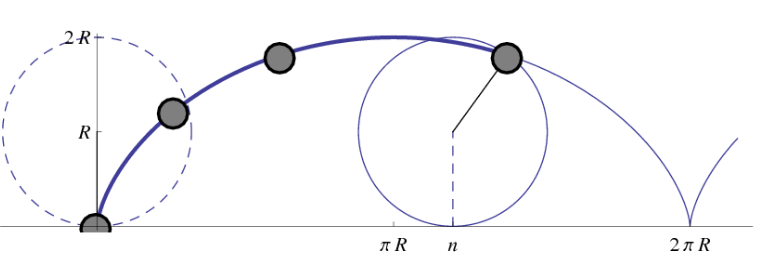
\includegraphics[scale=0.65]{picture1}

	\newpage\newpage
	\subsection*{Instrukcja obsługi}
	Aby uruchomić program należy otworzyć plik start.bat znajdujący się w głównym folderze projektu, następnie wybrać opcje Start wpisując 1 na klawiaturze oraz wcisnąć klawisz enter.
		
			
\includegraphics[scale=0.6]{instrukcja}

			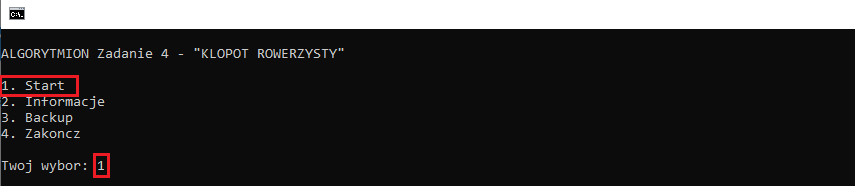
\includegraphics[scale=0.8]{instrukcja2}
	
	
\newpage
	\section*{Część II}
	\subsection*{Część techniczna}
Projekt obsługiwany jest z poziomu powłoki systemu Windows za pomocą pliku start.bat. Za pomocą tego skryptu uruchamiamy cały program, wyświetlamy informacje o projekcie, oraz możemy wyświetlić katalog backup. Po wybraniu opcji Start uruchamiany jest program server.exe, program ten został napisany w języku Java, plik .exe został wygenerowany za pomocą  aplikacji Launch4j. Server.exe jest swoistym głównym elementem całego projektu, tam wykonywane są operacje które spełniają warunki zadania z konkursu Algorytmion2014 tj.
obliczanie drogi jaką przebyła mucha (zakładając, że poruszała się ona na kole nie zmieniając na nim swojej pozycji) na podstawie danych wejściowych, które znajdowały się w plikach tekstowych w folderze input. Program zapisuje dane wyjściowe, wyniki do plików tekstowych w folderze output oraz na ich podstawie tworzy wykres prezentujący dane na wykresie słupkowym, który zapisywany jest w formacie png w celu późniejszego wykorzystania tego pliku graficznego.\\

Poźniej skrypt tworzy strukturę katalogów według daty rok-miesiąc-dzień, następnie kopiuje tam pliki projektu(wszystkie pliki z katalogu output, input, page.py, page.html, style.css, chart-date.png)\\

Kolejnym etapem jest uruchomienie przez skrypt start.bat skryptu page.py. Skrypt ten napisany w języku Python zbiera dane z wszystkich plików które obsługiwał wcześniej program server.exe następnie zapisuje je w pliku page.html. Zawartość plików .txt jest wyświetlana w formie tabeli według odpowiedniego klucza tj. w pierwszej kolumnie dane wejściowe z pliku input*.txt czyli, promień i dystans oraz w następnej kolumnie wynik, czyli droga jaką przebyła mucha z pliku output*.txt. Poniżej tabeli wyświetlany jest plik graficzny, który przedstawia wykres, który jest zestawieniem danych wejściowych i wyjściowych. Skrpt ten wymagał zebrania informacji z wielu plików została wykorzystana biblioiteka glob.\\


\\Ostatnim etapem jest uruchomienie pliku page.html co skutkuje otwarciem przeglądarki i wyświetleniem odpowiednich informacji. To jak powstaje ten plik oraz co zawiera zostało opisane w poprzednim akapicie. Za wygląd strony odpowiada pilik kaskadowego arkusza stylów style.css.  

	\newpage
	\subsection*{Opis działania} 
Główny algorytm oblicza drogę przebytą przez muche, która siedzi na kole. Dane wejściowe to promień koła oraz dystans przebyty przez koło. Droga przebyta przez muche jest obliczana z równania cykloidy.
Mamy funkcję getX i getY, które obliczają położenie muchy w danym momencie są to wzory:
$$x = r(t + sint)$$
$$y = r(1 - cost)\\$$

Zaczynamy od punktu $x_1=0$, $y_1=0$, $t=0$ i $x_2=getX(r, t)$, $y_2=getY(r, t)$. \\Wynik otrzymujemy z wzoru i dodajemy:
$$result+= \sqrt{(x_2-x_1)^2 + (y_2-y_1)^2}$$
Nastepnie naszym $x_1$ staje się punkt $x_2$, a $x_2$ pobieramy z funkcji getX w której argument t zwiększy się o 0.01 radiana. Analogicznie z punktami $y_1$ i $y_2$. Powyższe czynności wykonujemy dopóki $x_1$ zrówna się lub będzie większe od dystansu pobranego z pliku tekstowego.



	\subsection*{Implementacja}
Poniżej implementacja w formie pseudokodu odczytu danych z plików .txt, zapisu danych do pliku .txt, oraz algorytm, który spełnia warunki zadania Kłopot Rowerzysty z konkursu Algorytmion2014

	\begin{algorithm}[H]
	\SetKwData{Left}{left}\SetKwData{This}{this}\SetKwData{Up}{up}
	\SetKwInOut{Input}{input}\SetKwInOut{Output}{output}
	\caption{Odczyt danych z plików}
	\Input{Ścieżka do folderu z plikami .txt}
	\For{$Pliki w folderze$ \KwTo $Koniec folderu$}{
		\For{$Linia w Pliku$ \KwTo $EOF$}{
		$ListaPromieni$=+$Linia w Pliku$ \\
		$ListaDystansow$=+$Kolejna Linia w Pliku$}
		}
	\end{algorithm}
	
	\BlankLine
	
	\begin{algorithm}[H]
	\SetKwData{Left}{left}\SetKwData{This}{this}\SetKwData{Up}{up}
	\SetKwInOut{Input}{input}\SetKwInOut{Output}{output}
	
	\Input{wynik, nazwaPliku}
	
	\BlankLine
	
	Otwórz plik $nazwaPliku$ \\
	Wpisz $wynik$ do pliku $nazwaPliku$ \\
	Zamknij plik $nazwaPliku$
		\caption{Zapis danych do plików} \\
	\end{algorithm}
	
	\BlankLine
	
	\begin{algorithm}[H]
	\SetKwData{Left}{left}\SetKwData{This}{this}\SetKwData{Up}{up}
	\SetKwInOut{Input}{input}\SetKwInOut{Output}{output}
	\caption{Otrzymaj polozenie wspolrzednej X}
	\Input{promien, wartoscKata}
	\Output{wspolrzednaX}
	\BlankLine
	\Return $promien$ * ($wartoscKata$ - sinus($wartoscKata$))
	\end{algorithm}
	
	\BlankLine
	
	\begin{algorithm}[H]
	\SetKwData{Left}{left}\SetKwData{This}{this}\SetKwData{Up}{up}
	\SetKwInOut{Input}{input}\SetKwInOut{Output}{output}
	\caption{Otrzymaj polozenie wspolrzednej Y}
	\Input{promien, wartoscKata}
	\Output{wspolrzednaY}
	\BlankLine
	\Return $promien$ * (1 - cosinus($wartoscKata$))
	\end{algorithm}
	
	\BlankLine
	
	\begin{algorithm}[H]
	\SetKwData{Left}{left}\SetKwData{This}{this}\SetKwData{Up}{up}
	\SetKwInOut{Input}{input}\SetKwInOut{Output}{output}
	\caption{Otrzymaj wynik (Droga przebyta przez muche)}
	\Input{promien, dystans}
	\Output{wynik}
	\BlankLine
	$x1$ = 0, $x2$,
	$y1$ = 0, $y2$,
	$wartoscKata$ = 0, $wynik$ = 0  \Leftarrow Warunki początkowe \\
	\While{x1 < dystans} {
		$x2$ = otrzymajPolozenieX($promien$, $wartoscKata$) \\
		$y2$ = otrzymajPolozenieX($promien$, $wartoscKata$) \\
		$wynik += \sqrt{(x2-x1)^2 + (y2-y1)^2}$ \\
		$x1$ = $x2$ \\
		$y1$ = $y2$ \\
		$wartoscKata$ += 0.01 \\
		
	}

	\Return $wynik$
	\end{algorithm}
	\newpage
	\section*{Pełen kod programu}

	\begin{itemize}
	\item START.BAT
	\begin{lstlisting}
@echo off
title %Projekt Jezyki Skryptowe%


set mydateyear=%date:~6,4%
set mydatemonth=%date:~3,2%
set mydateday=%date:~0,2%

:main
cls
echo.
echo ALGORYTMION Zadanie 5 - "KLOPOT ROWERZYSTY"
echo.
echo 1. Start
echo 2. Informacje
echo 3. Backup
echo 4. Zakoncz
echo.
set /p answer="Twoj wybor: "
if %answer%==1 goto start
if %answer%==2 goto info
if %answer%==3 goto backup
if %answer%==4 goto end

:start
xcopy /Q /Y page.html .\backup\%mydateyear%\%mydatemonth%\%mydateday%\
xcopy /Q /Y style.css .\backup\%mydateyear%\%mydatemonth%\%mydateday%\
xcopy /Q /Y page.py .\backup\%mydateyear%\%mydatemonth%\%mydateday%\
xcopy /Q /Y .\input .\backup\%mydateyear%\%mydatemonth%\%mydateday%\
xcopy /Q /Y .\output .\backup\%mydateyear%\%mydatemonth%\%mydateday%\
xcopy /Q /Y .\images\chart_%mydateyear%_%mydatemonth%_%mydateday%.png .\backup\%mydateyear%\%mydatemonth%\%mydateday%\
start server.exe
start page.py
timeout 2 >nul
start page.html
goto main

:info
cls
echo Projekt Jezyki Skryptowe
echo ALGORYTMION Zadanie 5 - "KLOPOT ROWERZYSTY"
echo Arkadiusz Kaluza
echo Informatyka sem III, grupa 2C, RMS
pause
goto main

:backup
cls
dir .\backup /W
pause
goto main

:end
pause
echo on

	\end{lstlisting}
	
	\item PAGE.PY
	\begin{lstlisting}[language=Python]
import glob
from datetime import date

html = open("page.html", 'w', encoding="utf-8")
path_1 = "input/input_*.txt"
path_2 = "output/output_*.txt"
today = date.today()
d1 = today.strftime("%Y_%m_%d")

files_in = glob.glob(path_1)
files_out = glob.glob(path_2)

input = []
output = []

for name in files_in:
    with open(name) as f:
        word = f.readlines()
        input += word
        f.close()

inputString = ""
count = 0
for i in input:
    count += 1
    if count % 2 == 0:
        inputString += "D = " + str(i) + "\n"
    if count % 2 != 0:
        inputString += "R = " + str(i)

tab = inputString.splitlines()
for i in tab:
    if i == '':
        tab.remove('')
newTab = []
i = 0

for x in range(0, len(tab)):
    if len(tab) - 1 > i:
        newTab.append(tab[i] + ", " + tab[i + 1])
    i+=2

for name in files_out:
    with open(name) as f:
        word = f.readlines()
        output += word
        f.close()

html.write('<!DOCTYPE HTML>\n'
           '<html lang="pl">\n<head>'
           '    <meta charset="utf-8" />\n'
           '    <title>Jezyki Skryptowe Projekt</title>\n'
           '    <meta name="descripton" content="Projekt Języki Skryptowe Arkadiusz Kałuża"/>\n'
           '    <meta http-equiv="X-UA-Compatible" content="IE=edge,chrome=1"/> \n'
           '    <link rel="stylesheet" href="style.css" type="text/css" /> \n'
           '    <link href="https://fonts.googleapis.com/css?family=Lato&display=swap" rel="stylesheet"> \n'
           '</head> \n'
           '<body> \n'
           '    <div id="container"> \n'
           '        <div id="header"> \n'
           '            "KŁOPOT ROWERZYSTY" - Algorytmion 2014 \n         '
           '        </div> \n'
           '        <div id="content"> \n'
           '            <div id="tab">\n'
           '                <table>\n'
           '                    <tr>\n'
           '                        <th>Promień i Dystans</th>\n'
           '                        <th>Droga przebyta przez muche</th>\n'
           '                    </tr>\n')
i = 0
j = 0


while (i != len(tab) and j!=len(output)):
    html.write('                 <tr>\n                     '
               '                       <td>')
    html.write(newTab[i].replace('\n', ''))
    html.write('</td>\n                     <td>')
    html.write(output[j].replace('\n', ''))
    html.write('</td> \n                 </tr>\n')
    i += 1
    j += 1

html.write('                </table>\n'
           '            </div>\n'
           '            <div id="txt">Ponizej zestwaienie danych wejsciowych i wyjsciowych </div> \n'
           '            <img src="images/chart_' + d1 + '.png"/>\n'
           '           </div> \n'
           '           <div id="footer"> \n'
           '                &copy Arkadiusz Kałuża, RMS POLSL \n'
           '           </div> \n'
           '    </div> \n'
           '</body> \n')
html.close()
	\end{lstlisting}
	
	\item PAGE.PY
	\begin{lstlisting}[language=Python]
import glob
from datetime import date

html = open("page.html", 'w', encoding="utf-8")
path_1 = "input/input_*.txt"
path_2 = "output/output_*.txt"
today = date.today()
d1 = today.strftime("%Y_%m_%d")

files_in = glob.glob(path_1)
files_out = glob.glob(path_2)

input = []
output = []

for name in files_in:
    with open(name) as f:
        word = f.readlines()
        input += word
        f.close()

inputString = ""
count = 0
for i in input:
    count += 1
    if count % 2 == 0:
        inputString += "D = " + str(i) + "\n"
    if count % 2 != 0:
        inputString += "R = " + str(i)

tab = inputString.splitlines()
for i in tab:
    if i == '':
        tab.remove('')
newTab = []
i = 0

for x in range(0, len(tab)):
    if len(tab) - 1 > i:
        newTab.append(tab[i] + ", " + tab[i + 1])
    i+=2

for name in files_out:
    with open(name) as f:
        word = f.readlines()
        output += word
        f.close()

html.write('<!DOCTYPE HTML>\n'
           '<html lang="pl">\n<head>'
           '    <meta charset="utf-8" />\n'
           '    <title>Jezyki Skryptowe Projekt</title>\n'
           '    <meta name="descripton" content="Projekt Języki Skryptowe Arkadiusz Kałuża"/>\n'
           '    <meta http-equiv="X-UA-Compatible" content="IE=edge,chrome=1"/> \n'
           '    <link rel="stylesheet" href="style.css" type="text/css" /> \n'
           '    <link href="https://fonts.googleapis.com/css?family=Lato&display=swap" rel="stylesheet"> \n'
           '</head> \n'
           '<body> \n'
           '    <div id="container"> \n'
           '        <div id="header"> \n'
           '            "KŁOPOT ROWERZYSTY" - Algorytmion 2014 \n         '
           '        </div> \n'
           '        <div id="content"> \n'
           '            <div id="tab">\n'
           '                <table>\n'
           '                    <tr>\n'
           '                        <th>Promień i Dystans</th>\n'
           '                        <th>Droga przebyta przez muche</th>\n'
           '                    </tr>\n')
i = 0
j = 0


while (i != len(tab) and j!=len(output)):
    html.write('                 <tr>\n                     '
               '                       <td>')
    html.write(newTab[i].replace('\n', ''))
    html.write('</td>\n                     <td>')
    html.write(output[j].replace('\n', ''))
    html.write('</td> \n                 </tr>\n')
    i += 1
    j += 1

html.write('                </table>\n'
           '            </div>\n'
           '            <div id="txt">Ponizej zestwaienie danych wejsciowych i wyjsciowych </div> \n'
           '            <img src="images/chart_' + d1 + '.png"/>\n'
           '           </div> \n'
           '           <div id="footer"> \n'
           '                &copy Arkadiusz Kałuża, RMS POLSL \n'
           '           </div> \n'
           '    </div> \n'
           '</body> \n')
html.close()

	\end{lstlisting}
	
	\item PAGE.HTML
	\begin{lstlisting}[language=Html]
<!DOCTYPE HTML>
<html lang="pl">
<head>    <meta charset="utf-8" />
    <title>Jezyki Skryptowe Projekt</title>
    <meta name="descripton" content="Projekt Języki Skryptowe Arkadiusz Kałuża"/>
    <meta http-equiv="X-UA-Compatible" content="IE=edge,chrome=1"/> 
    <link rel="stylesheet" href="style.css" type="text/css" /> 
    <link href="https://fonts.googleapis.com/css?family=Lato&display=swap" rel="stylesheet"> 
</head> 
<body> 
    <div id="container"> 
        <div id="header"> 
            "KŁOPOT ROWERZYSTY" - Algorytmion 2014 
                 </div> 
        <div id="content"> 
            <div id="tab">
                <table>
                    <tr>
                        <th>Promień i Dystans</th>
                        <th>Droga przebyta przez muche</th>
                    </tr>
                 <tr>
                                            <td>R = 2, D = 1</td>
                     <td>2.146486813203168</td> 
                 </tr>
                 <tr>
                                            <td>R = 6, D = 12</td>
                     <td>17.118817137095423</td> 
                 </tr>
                 <tr>
                                            <td>R = 43, D = 23</td>
                     <td>48.51931428849752</td> 
                 </tr>
                </table>
            </div>
            <div id="txt">Ponizej zestwaienie danych wejsciowych i wyjsciowych </div> 
            <img src="images/chart_2019_12_30.png"/>
           </div> 
           <div id="footer"> 
                &copy Arkadiusz Kałuża, RMS POLSL 
           </div> 
    </div> 
</body> 
	\end{lstlisting}
	
	\item STYLE.CSS
	\begin{lstlisting}
body
{
    margin: 0 !important;
    background-color: #3a565e;
    font-family: 'Lato', sans-serif;

}
table
{
    width: 100%;
    border-collapse: collapse;
    margin-left: auto;
    margin-right: auto;
    border: 3px solid #dad9d9;
}
td, th
{
    padding: 8px;
    border: 1px solid #dad9d9;

}
th
{
    text-align: center;
    border-bottom: 3px solid #dad9d9;
    background-color:  #3a565e;
}
td
{
    text-align: left;
}
#tab
{
    padding: 15px;
    margin-left: auto;
    margin-right: auto;
    overflow-x: auto;
}
#container
{
    width: 100%;

}
#header
{

    width: 100%;
    padding: 15px 0;
    background-color: #5e8691;
    color: whitesmoke;
    text-align: center;
    font-size: 20px;
}
#content
{
    min-height: 905px;
    width: 1000px;
    margin-left: auto;
    margin-right: auto;
    text-align: justify;

    background-color: #5d6a6e;
    color: whitesmoke;

}

#footer
{

    text-align: center;
    padding: 10px;
    background-color: #5e8691;
}
#txt
{
    font-size: 20px;
    text-align: center;
    padding-bottom: 15px ;
}

img {
    display: block;
    margin-left: auto;
    margin-right: auto;
    padding-bottom: 15px;
  }


	\end{lstlisting}

	\item Rowerzysta.java
	\begin{lstlisting}
	import java.io.*;
import java.util.Scanner;
import org.jfree.chart.*;
import org.jfree.chart.plot.PlotOrientation;
import org.jfree.data.category.CategoryDataset;
import org.jfree.data.category.DefaultCategoryDataset;
import java.time.format.DateTimeFormatter;
import java.time.LocalDateTime;

public class Rowerzysta {
    public JFreeChart createChart(int height, int width, String chartTitle, double[] radiusValues, double[] distanceValues, double[] resultValues) {
        JFreeChart barChart = ChartFactory.createBarChart(
                chartTitle,
                "Category",
                "Score",
                createDataset(radiusValues, distanceValues, resultValues),
                PlotOrientation.VERTICAL,
                true, true, false);
        ChartPanel chartPanel = new ChartPanel(barChart);
        chartPanel.setPreferredSize(new java.awt.Dimension(width , height));

        return barChart;
    }

    private CategoryDataset createDataset(double[] radiusValues, double[] distanceValues, double[] resultValues) {
        int length = radiusValues.length;
        final DefaultCategoryDataset dataset = new DefaultCategoryDataset();
        String label1 = "";
        String label2 = "";
        String label3 = "";

        for(int i = 0; i < length; i++) {
            label1 = "Radius" + Integer.toString(i);
            label2 = "Distance" + Integer.toString(i);
            label3 = "Results" + Integer.toString(i);
            dataset.addValue(radiusValues[i], label1, "Radius");
            dataset.addValue(distanceValues[i], label2, "Distance");
            dataset.addValue(resultValues[i], label3, "Results");
        }
        return dataset;
    }

    public double getX(double r, double t) {
        return r * (t - Math.sin(t));
    }

    public double getY(double r, double t) {
        return r * (1 - Math.cos(t));
    }

    public double getResult(double radius, double distance) {
        double x1 = 0, x2;
        double y1 = 0, y2; 
        double t = 0;
        double result = 0;
        while (x1 < distance) {
            x2 = getX(radius, t);
            y2 = getY(radius, t);
            result += Math.sqrt(Math.pow((x2 - x1), 2) + Math.pow((y2 - y1), 2));
            x1 = x2;
            y1 = y2;
            t += 0.01; // zwiększenie kata o stala wartosc 0.01rad
        }
        return result;
    }

    public void writeResultToFile(double result, String outputFileName) throws FileNotFoundException {
        PrintWriter out = new PrintWriter("./output/" + outputFileName);
        String output = Double.toString(result);
        out.write(output);
        out.close();
    }

    public File[] getFilesInDirectory(String pathInput) {
        File dir = new File(pathInput);
        File[] filesInDirectory = dir.listFiles();
        return filesInDirectory;
    }

    public static String getStringDate() {
        DateTimeFormatter dtf = DateTimeFormatter.ofPattern("yyyy_MM_dd");
        LocalDateTime now = LocalDateTime.now();
        String date = dtf.format(now);
        return date;
    }

    public static void main(String[] args) throws FileNotFoundException, IOException {
        Rowerzysta rowerzysta = new Rowerzysta();
        String pathInput = "./input/";
        File[] filesInDirectory = rowerzysta.getFilesInDirectory(pathInput);
        double[] radiusValues = new double[filesInDirectory.length];
        double[] distanceValues = new double[filesInDirectory.length];
        double[] resultsValues = new double[filesInDirectory.length];

        int count = 0;
        for(File f : filesInDirectory) {
            File file = new File(pathInput + f.getName());
            Scanner in = new Scanner(file);
            try{
                double radius = in.nextDouble();
                double distance = in.nextDouble();
                double result = rowerzysta.getResult(radius, distance);
                radiusValues[count] = radius;
                distanceValues[count] = distance;
                resultsValues[count] = result;
                count++;
                String outputFileName = "output_" + count + ".txt";
                rowerzysta.writeResultToFile(result, outputFileName);
            } catch (Exception e) {
                System.out.println("Error: " + e);
            }
            in.close();
        }
        JFreeChart chart = rowerzysta.createChart(650, 600, "Chart", radiusValues, distanceValues, resultsValues);
        ChartUtilities.saveChartAsJPEG(new File("./images/chart_" + getStringDate() + ".png"), chart, 600, 650);
    }
}

	\end{lstlisting}
	\end{itemize}

\end{document}